\section{冻结规则以后，材料步改善是否仍然出现}
我先用平滑Gaussian、近接触Gaussian、分层体素（voxel）和非对称voxel四个对象检查方法，分别取初始化、保存迭代索引3和最后保存的状态，再比较$k=4,8,16$。这36个单元中35个改善、1个保持相同；四个对象先各自求和再比较，中位完整GN gap下降65.2\%。这里九个状态和预算组合仍属于一个对象，我没有把它们当成九个独立样本。

随后我锁定全部规则和数值阈值，检查资产中其余所有兼容对象。十个对象完整提供各九个单元，十个都改善；中位风险比0.4928，即下降50.7\%，四分位区间[0.3314,0.5588]。按对象重采样（object bootstrap）得到的中位数95\%区间为[0.3133,0.5647]。还有一个非对称voxel对象的中期以前六个单元改善，但晚期receiver endpoint在第一个预算没有通过预设法方程残差（normal residual）检查，后面两个预算未运行。因此预定99个单元只有96个有有效结果，失败仍在总表中。

\begin{figure}[htbp]\centering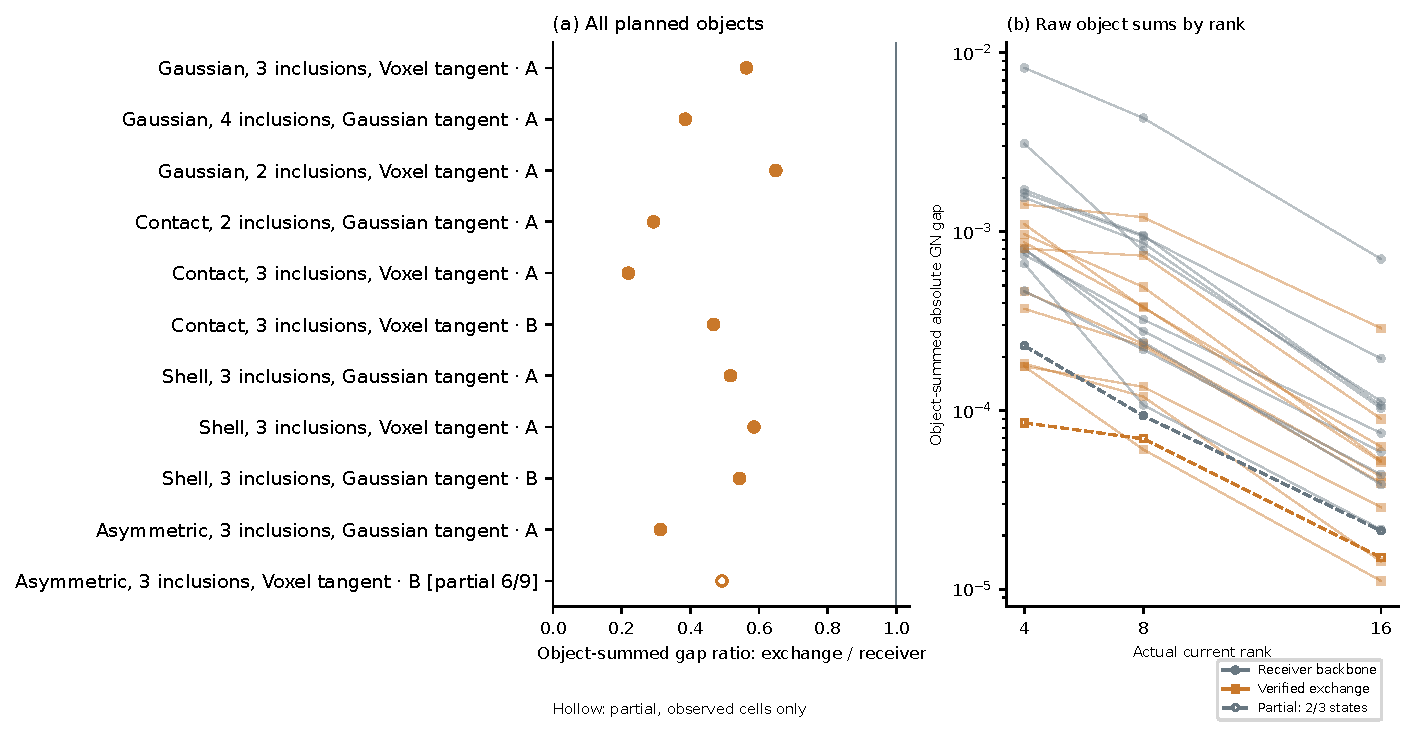
\includegraphics[width=.96\linewidth]{figures/closure_validation_v2/Figure1_primary_overview.pdf}
\caption{左图逐对象展示完整GN gap之和的比值，右图展示不同实际电流秩下的绝对gap。空心点和虚线单独标出只有六个可用单元的对象。这张图检验材料步保真度，不是最终材料图像。}
\end{figure}

这个结果比较有说服力的地方是，效果不只来自原四个对象，也不只来自小分母：最小receiver gap仍超过evaluation floor约$6.31\times10^9$倍。96个有效单元中95个改善、1个相同，绝对下降量和$H$范数步误差都有逐项记录。不过，这些对象曾进入宽域current-ranking研究，无法确认它们完全没有影响过历史规则判断。因此我把它们称为冻结规则在额外对象上的检验，避免把它写成全新blind dataset。

\section{加噪声以后，收益保留，但电流方向会改变}
我按几何和材料表示事先选了四个对象：平滑voxel、接触Gaussian、壳体Gaussian和非对称voxel。固定中期物理状态，在1\%和3\%复噪声下各用三份独立噪声样本（realization），再比较三个电流秩。每份噪声都有自己的完整GN reference，因为残差改变，材料步的比较目标也随之改变。

72个单元全部完成，71个改善、1个保持原空间。四对象汇总风险比的中位数在1\%时为0.3307，在3\%时为0.4026。这个有限噪声测试支持材料步收益仍然存在。它没有要求选择同一组电流：用主角度（principal angle，衡量两个物理子空间的偏离）比较保存的空间，很多补入方向明显改变。因此更合适的理解是，方法追随当前残差选择有用的变化，而不是得到一个不随数据改变的稳定模式表。

完整复核检查408个finalist，其中98个低于数值接受阈值，共接受172次交换。Jd核验用了2448个电流方程右端（current right-hand sides, RHS），包括被拒绝的候选。已有缓存后的评分（warm scoring）只是其中一个阶段，完整费用还包括取得候选与物理检查。

\subsection{好方向是否进入了候选池？}
为了区分“评分不准”和“没有送来好候选”，我在已完成线上决定以后，离线枚举固定154方向字典中的全部初次一换一机会（initial one-exchange opportunity），再走最多三个按完整收益选择的局部动作。这个teacher只作诊断，没有回传到线上规则。96个可用单元完整，之前端点失败对应的3个单元仍未运行。

在十个完整额外对象中，如果允许anchor在全字典排序，它保留的初次正收益机会为97.30--99.99\%，中位99.54\%。但是固定12个移入候选的短池只覆盖49.12--95.31\%，中位72.95\%。这些比例先对对象内机会求和，因此我把目前更明显的瓶颈理解为候选取得（candidate acquisition），而不是排序公式本身。这并不表示已经解决全局选模：后续交换进入不同条件空间，局部路径也会不同。完整收益贪心路径在90个单元终态更好，线上路径在5个单元更好，1个在评价底噪内相同；这个差距包含覆盖、排序与路径共同作用。


\subsection{把规则放回真正的约束反演以后}
我还固定四个代表对象，把receiver和exchange放进相同的outer reconstruction：同一初始化、prior、LM schedule、材料可行域以及完整非线性目标上的Armijo line search，只改变切向电流策略。三个完整对照都完成18次接受更新。平滑voxel、近接触Gaussian和shell Gaussian的复材料相对误差分别从0.3027、0.6722、0.6096降到0.2699、0.6707、0.5660，约下降10.8\%、0.22\%、7.16\%。留出测量误差也均下降。

这里有一个值得正面解释的差别：近接触对象的数据拟合改善很明显，但复材料改善很小，实部还略差。这使我更明确地区分“更忠实的完整GN步”和“更好的材料估计”。第四个非对称voxel对象的exchange轨迹保留17次已完成更新。在第18次更新前，它为开始当次交换构建的receiver endpoint没有通过残差验收，因而停止；独立的receiver-only基线轨迹尚未运行。我保留这组未形成完整对照的结果，没有放宽验收条件。

每条轨迹独立计入setup、acquisition、line search和最终评价后，exchange耗时是receiver的2.68、1.74、1.46倍。它支付了额外的$Jd$作用，换取更新保真度，而不是更快的成像。我的论文因此以Maxwell机制和conditional design为主，把这三组重建作为有限的secondary consequence。

\begin{figure}[htbp]\centering
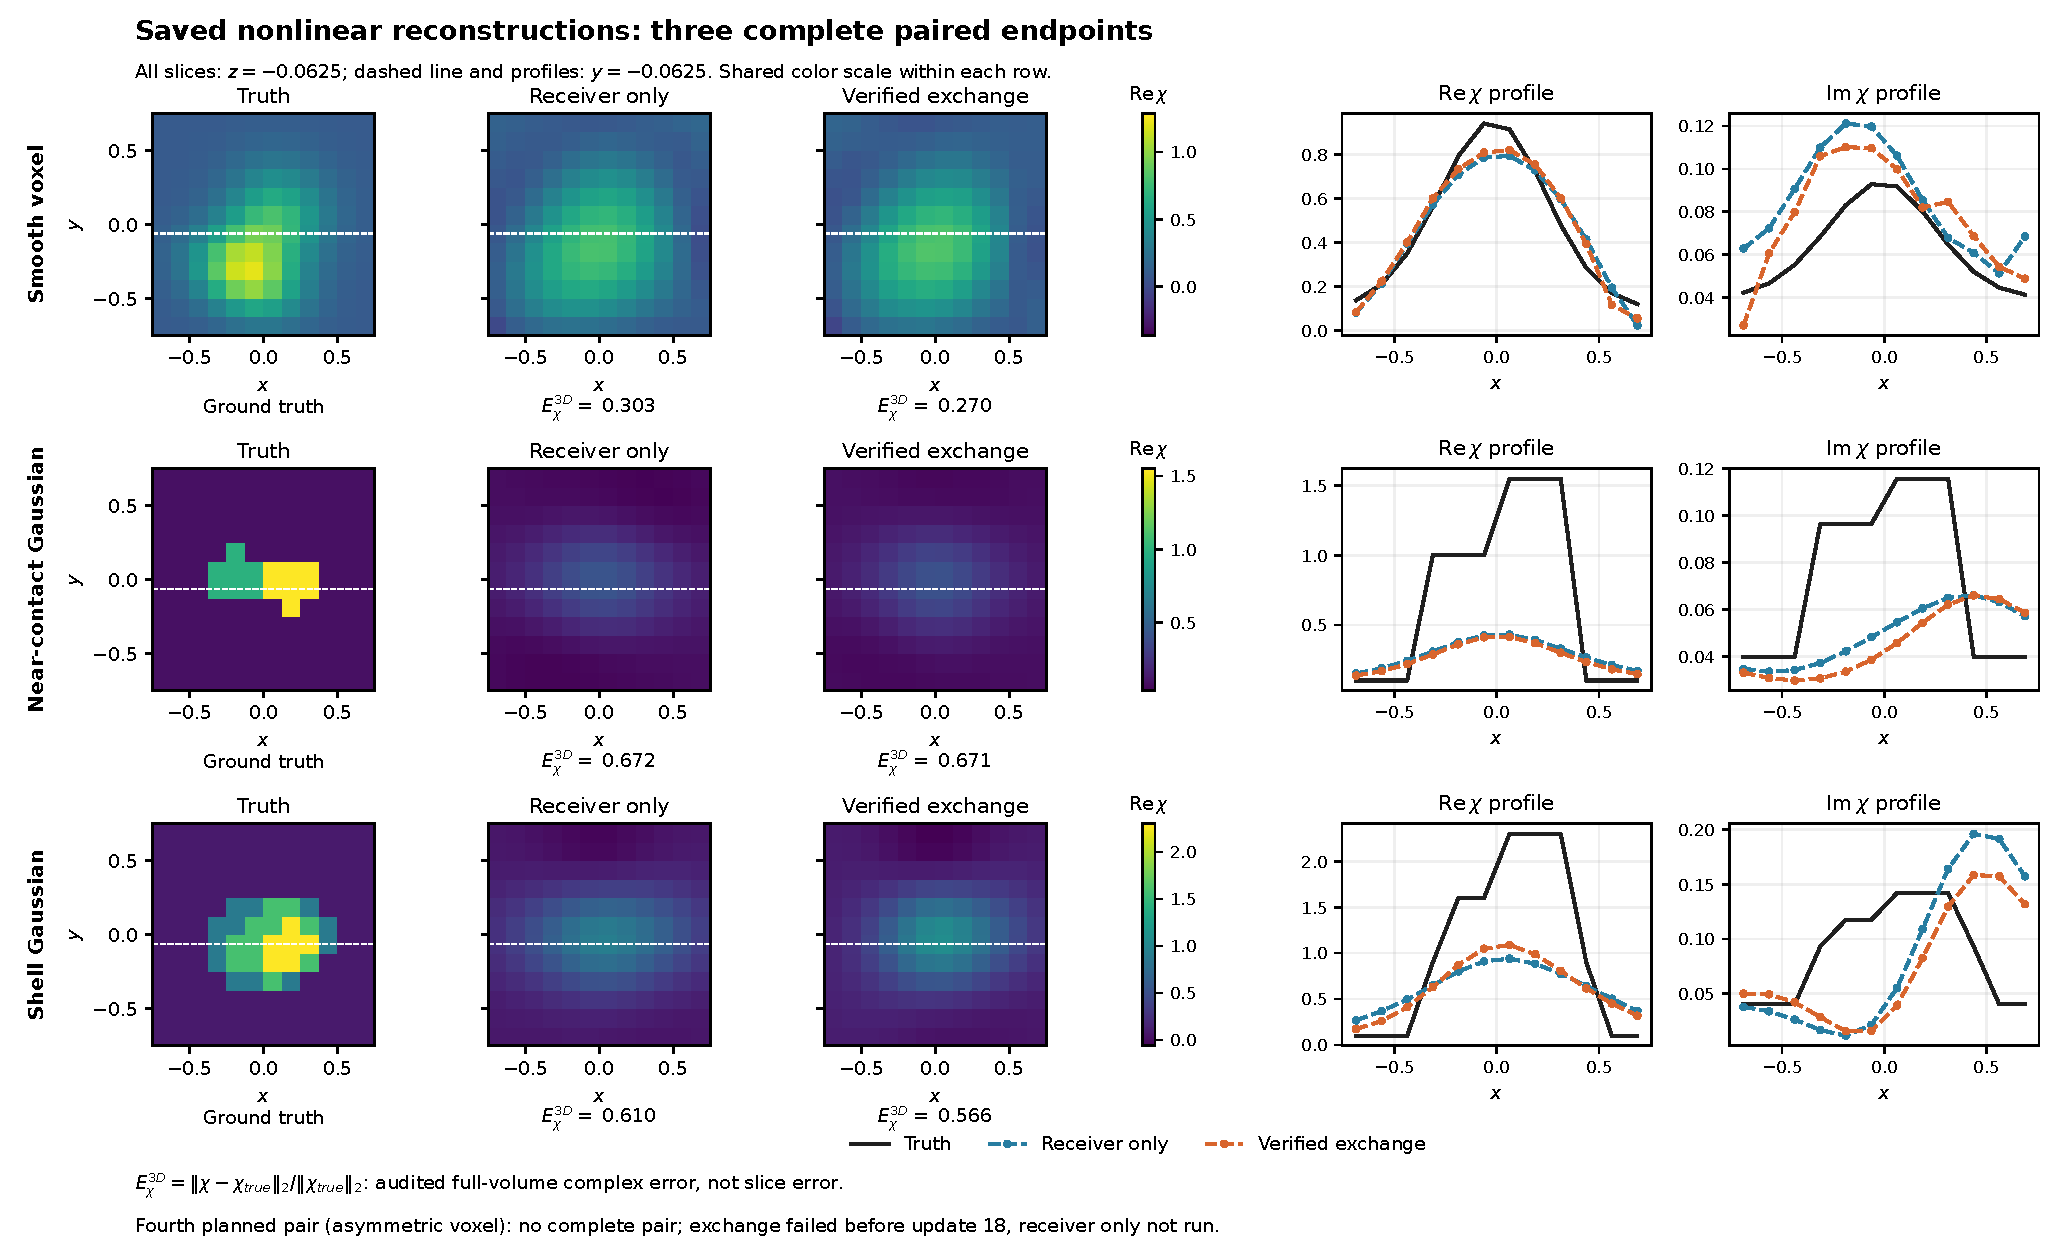
\includegraphics[width=.95\linewidth]{figures/nonlinear_closure_v1/nonlinear_reconstructions.pdf}
\caption{三组完整对照的材料切片与剖面。每行共用色标，曲线同时展示实部和虚部；完整误差用整个三维材料计算。近接触及shell结构的峰值和界面仍不清晰，数据拟合改善没有自动解决材料辨识。}
\end{figure}


\subsection{改善的代价如何理解}
我把费用分成共同物理计算、anchor与候选取得、排序、完整方向核验、离线诊断和真正重建，拒绝动作和失败也计入。整个研究的已计费作业占用为5.545小时；这个数是执行账本，不能当成一次反演的时间。冻结流程重用共同算子，数秒的warm选择也不能代表冷启动。

三对独立重建的exchange耗时为receiver的2.68、1.74和1.46倍。因此我的结果是用额外物理作用换取材料步保真度，并在部分对象看到有限重建后果。它没有给出加速成像结论。每个finalist的复核只需要完整$Jd$，省掉的是这项判断中的新增伴随（adjoint），并没有省掉取得候选和验证所需的全波计算。


